\chapter{System Design}
This chapter details about how the above technologies are integrated into one system. It discusses each component in depth e.g. explaining how they link the system together.

\section{Design Overview}
The system architecture consists of three main areas. A web application, which connects to a server via an API and finally the server connecting to a database. The server acts as a line of communication between the web application and the database. The server also carries out any necessary calculations that are needed on sent or retrieved data.\par
The elements were chosen based on the client needs as well as creating a challenging project. It would have been much simpler to choose a traditional stack e.g. MEAN, but already having experience using this method, felt choosing a custom stack would test my abilities to a higher level.\par
Although not a traditional stack for web applications in industry, learning these was a useful skill as they are some of the fastest growing technologies in the area of web applications.
\newpage
\begin{figure}[h!]
 	\caption{System Design Architecture}
	\label{image:projectdesign}
 	\centering
 	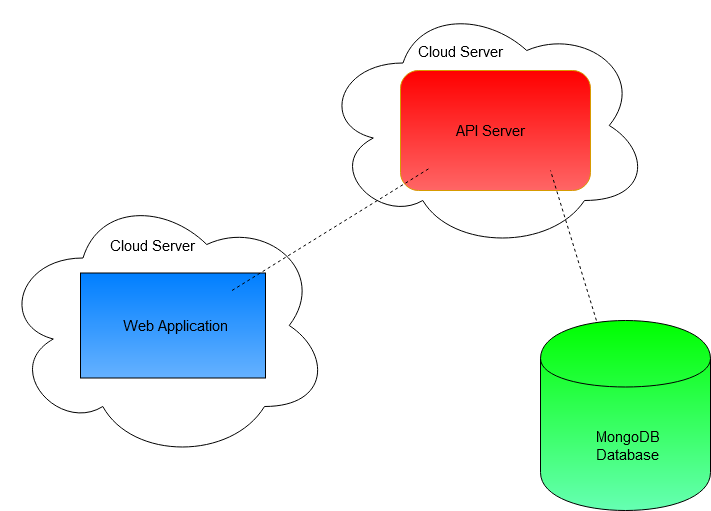
\includegraphics[width=0.9\textwidth]{Images/Project Layout.png}
\end{figure}

\section{Revenue Computation Process}
This section gives a very brief summary of the process of how the revenue system is carried out and calculated within the brewing industry. Each beer has its own container within each section of the detailed below headings in Figure \ref{fig:revenuecomp}. It also details the complexity within the computation process, as well as showcasing the areas which require manual entry of data to produce the automatically calculated data.
\begin{figure}[h!]
 	\caption{Revenue Computation Diagram}
	\label{fig:revenuecomp}
 	\centering
 	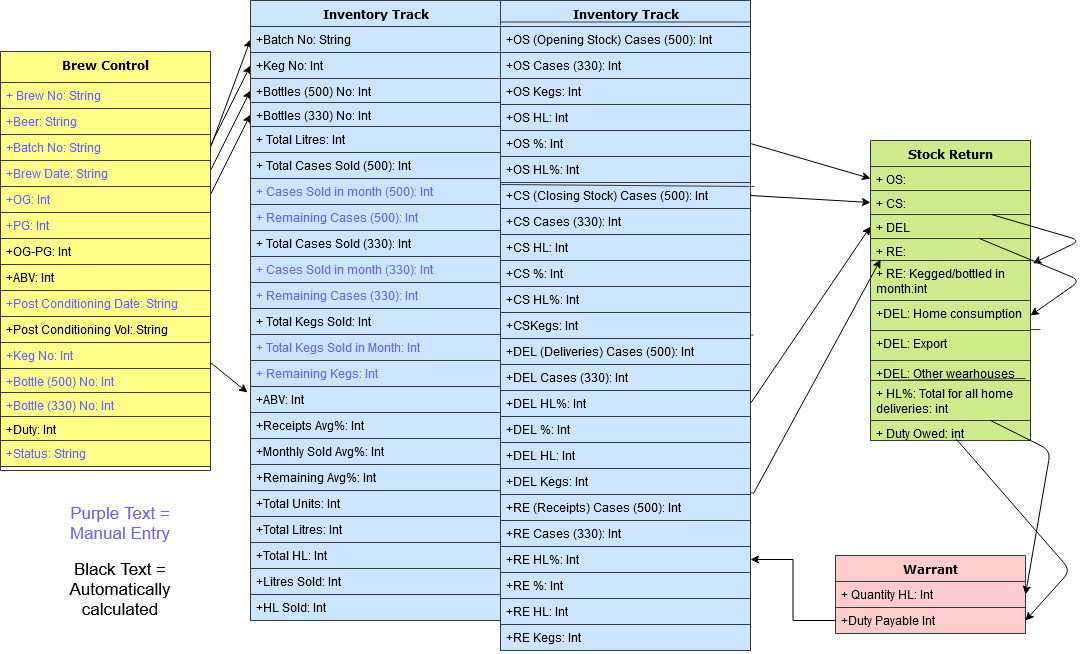
\includegraphics[width=1.25\textwidth]{Images/API Design.png}
\end{figure}
\newpage

\subsection{Brews}
The first step is brewing the beer, this results in each brew having its own unique batch number. Each brew has many different calculations which need to be entered, original gravity, ABV(Alcohol by volume) percentage etc. The purpose of keeping records of these is to calculate inventories and keep a record of each batch of beer brewed by the brewery.

\subsection{Inventories}
The inventories are then calculated, these are dependent on a brew as well as its own data entries in order to calculate the values needed to produce all necessary values. This section contains the largest amount of data to be calculated and stored. The purpose of keeping these inventories is to record sold and remaining stock. During the Inventory calculations, receipts, deliveries and closing stock numbers are all calculated. These numbers are then sent to revenue. Inventories are also used to calculate stock returns.

\subsection{Stock Returns}
The purpose of the Stock Returns is to create a table of calculations and percentages that are required to be sent to revenue. Stock Returns take into account all of the inventories for a specific beer within a monthly period rather than a single batch number.

\subsection{Warrants}
Warrants are calculated using a stock return of a beer. These are then printed out, signed and sent with the required figures to revenue. 

\section{Web Application}
The web application was the first component to be designed, this was due to it being the most important part from the clients perspective. The main features of the web application were that it had to have forms with which the user could enter the least amount of data possible for each section. They also needed then to access the processed data with the new data calculated from their inputs. These all need to be readable, updateable and deletable. The data must also be sortable by month. This is important as revenue must be updated on a monthly basis and the client needs to be able to check on previous months' brews, inventories etc. The web application also contains a login page which ensures the user is logged in to access data. React also allows you to block access to pages when the user is not authenticated, this is possible due to the ability to install external libraries which implement components which grant this functionality. Okta libraries were used in the case of this project to restrict page availability. \par
The web application consists of many different components which need to interact with each other in order for the application to function. The main components are as follows:
\begin{itemize}
    \item Login Component.
    \item Home Component with links to other components.
    \item Individual forms Components to create brews, inventories, stock returns and warrants.
    \item Individual filter Components to access each of above by beer, batch number where valid and month.
    \item Components to access each individual data entry with the ability to update, delete and print information to PDF or direct to a printer.
    \item Component to create and update brewer information.
\end{itemize}
\begin{figure}[h!]
 	\caption{Web Application Design Architecture}
	\label{image:webappdesign}
 	\centering
 	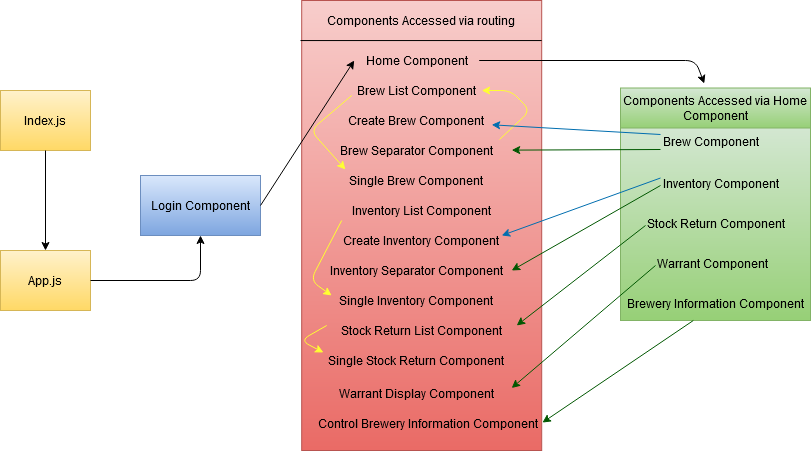
\includegraphics[width=1\textwidth]{Images/React Structure.png}
\end{figure}
The web application must communicate with the server to send and receive data in JSON format. It must also send validation that the user is authorized to push or pull data from the server using a web token. \par
The form pages allow users to input relevant data which is needed to record a full set of calculations to a data entry of the form type they are submitting e.g a brew or inventory. User data entries are sent to the server to have computations carried out on them. There are user forms for creating new entries as well as the ability to update existing data entry values. Pages which allow users to update data automatically populate the form with the current matching data associated with that entry.\par
\begin{figure}[h!]
 	\caption{Example of an update form in the Web Application}
	\label{image:form}
 	\centering
 	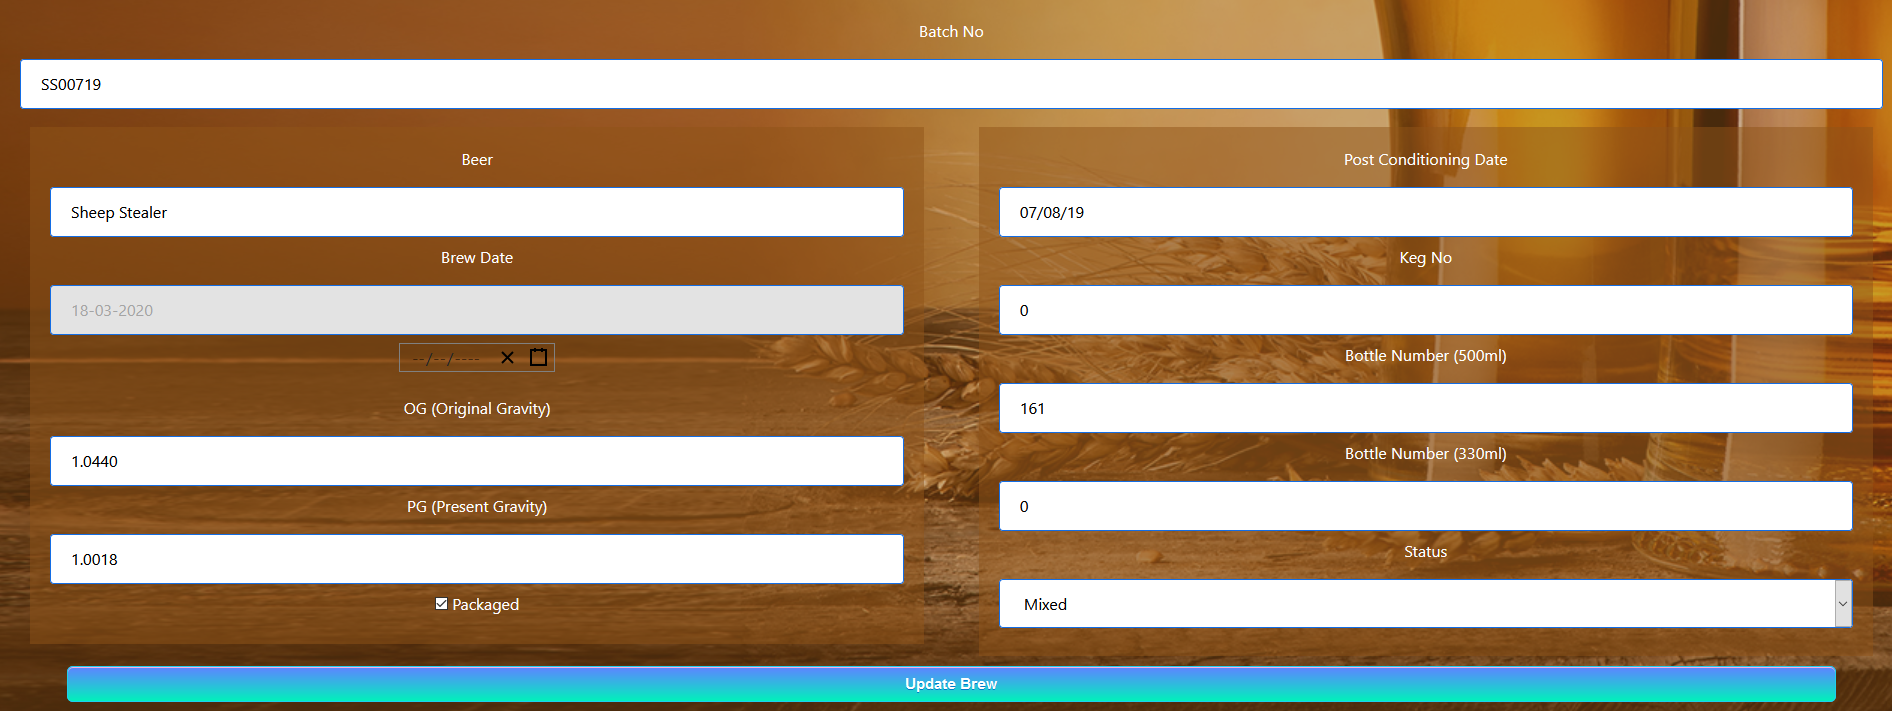
\includegraphics[width=1\textwidth]{Images/form.PNG}
\end{figure}
All data entries can be sorted by month. This means the user can select a month they wish to view data entries from and access them. This is crucial as it allows the brewer to access all entries of a beer for a specific month which is how revenue groups them together. A feature like this easily allows users to see data entries that were set within that period. \\
\begin{figure}[h!]
 	\caption{Example of Data Sorting}
	\label{image:datasorting}
 	\centering
 	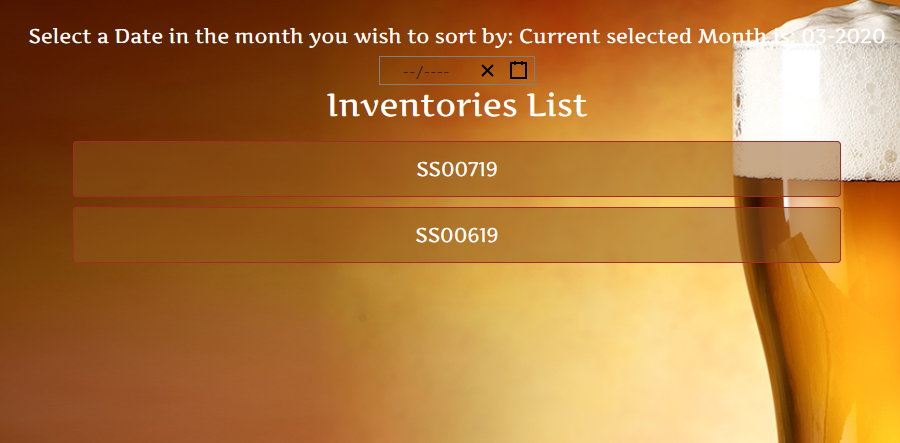
\includegraphics[width=1\textwidth]{Images/sorting.PNG}
\end{figure}
\newpage
Data entries all have different variations of data viewing pages depending on the formula the data is required in by revenue i.e. data needs to be presented differently in stock returns than in an inventory etc. All calculation data viewing pages give the user options to delete the data or print the data to a PDF or directly to a printer. All calculation data viewing pages except stock returns give the user an edit data option which displays a form below the data which as stated above can update data entries. Stock returns use all inventory data of a specific beer so therefore cannot be updated manually. 

\begin{figure}[h!]
 	\caption{Example of data display of a Stock Return}
	\label{image:datadisplay}
 	\centering
 	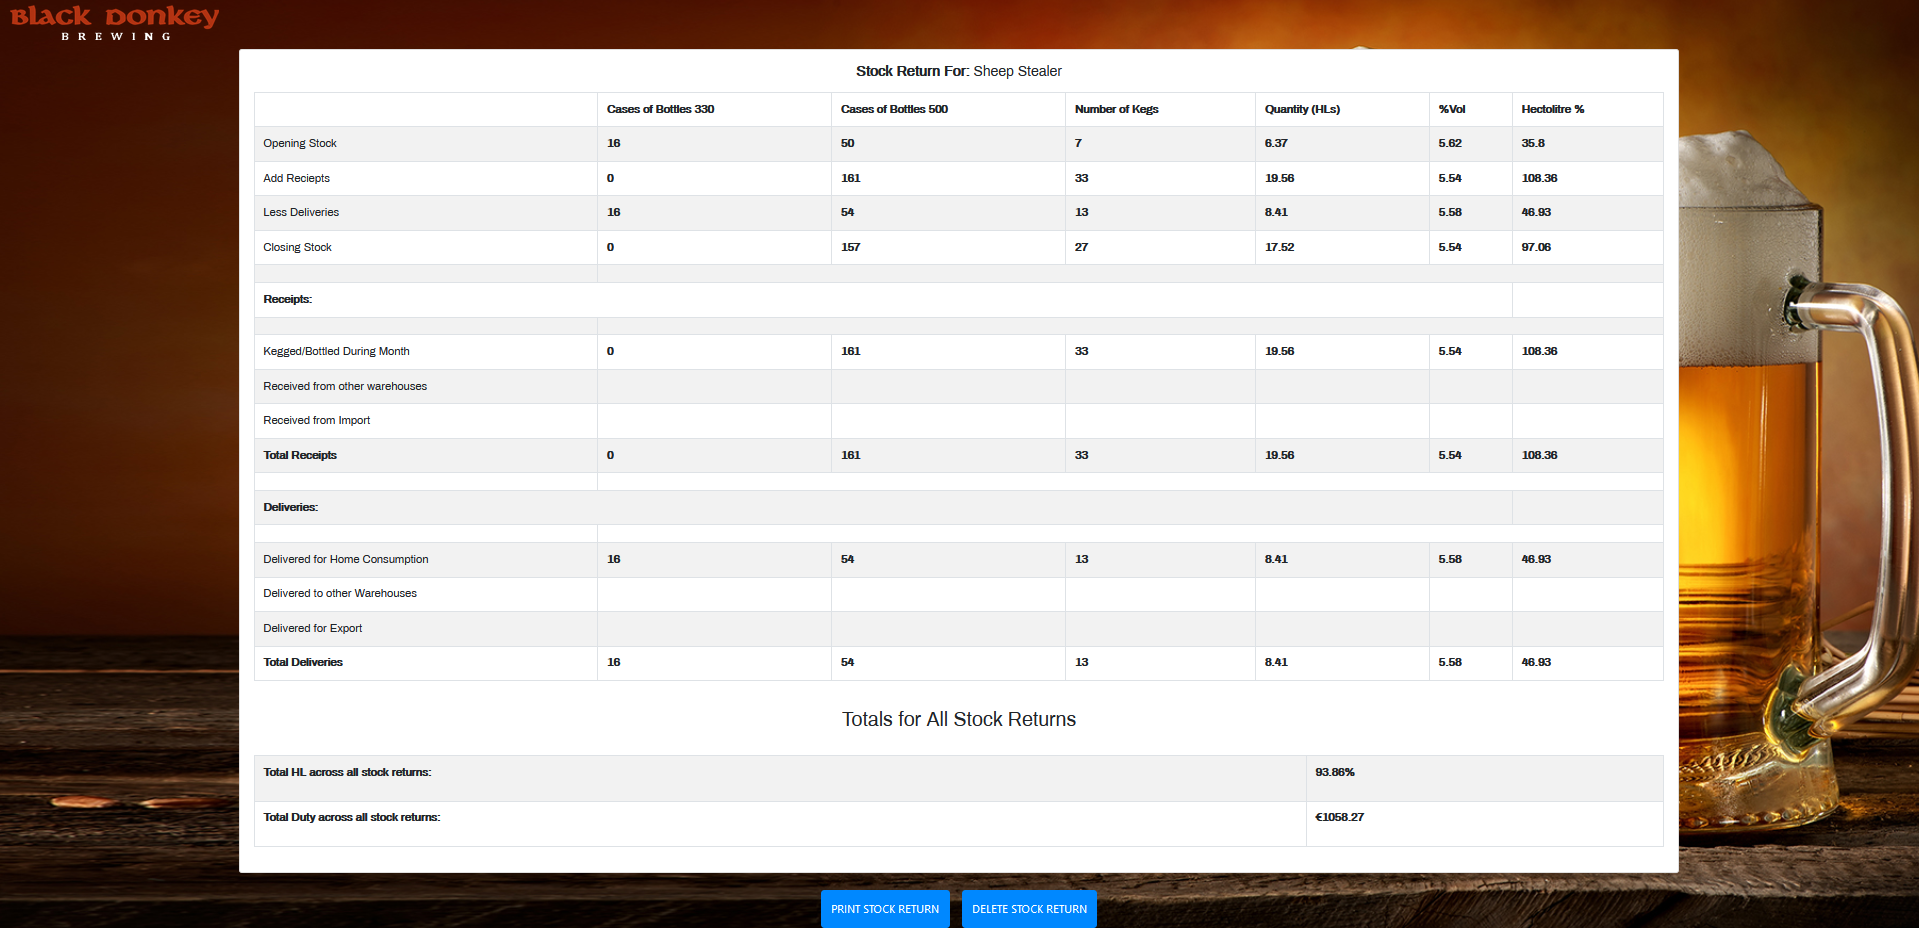
\includegraphics[width=1\textwidth]{Images/dataexample2.PNG}
\end{figure}
\newpage

\section{API Server}
The API server acts as a line of communication between the web application and the database. The API ensures that user sent data is processed. The data sent must go through a calculation process. The newly calculated data is then sent to the database to be stored. The API also handles sending back this data to the web application for user display. No data processing will take place unless the server has authenticated the request, meaning no user outside the application can access data without a valid token. \par
The API server is run using Flask, this was chosen due to its scalability, adaptability, reliability and because it’s a lightweight framework. Flask is also easily testable using programs such as Postman which was used throughout development. Flask also carries out requests at high speeds which is very important for the user's experience.\par
The API was designed in a RESTful manner which meant that managing a user session was not necessary. This speeds up the server as it may take time to store user session info and check on every request. REST also uses standard HTTP requests making the communication process much simpler with the web application and the API. The API was designed in a RESTful manner which meant that managing a user session was not necessary. This speeds up the server as it may take time to store user session info and check on every request. REST also uses standard HTTP requests making the communication process much simpler with the web application and the API. GET, POST, PUT and DELETE requests are all handled at the server’s URL addresses at different endpoints for brews, inventories, stock returns and brewery information respectively.
\begin{figure}[h!]
 	\caption{Server Design Architecture}
	\label{image:serverdesign}
 	\centering
 	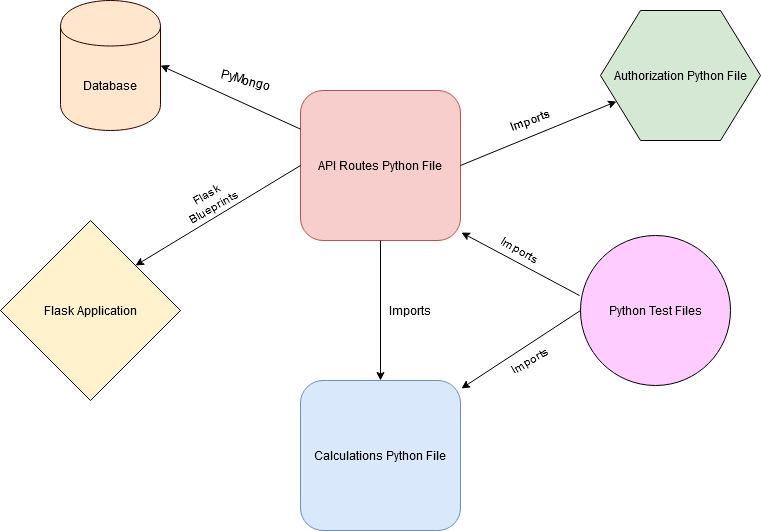
\includegraphics[width=1\textwidth]{Images/Server Structure.png}
\end{figure}
\begin{figure}[h!]
 	\caption{Server Class Diagram}
	\label{image:serverdiagram}
 	\centering
 	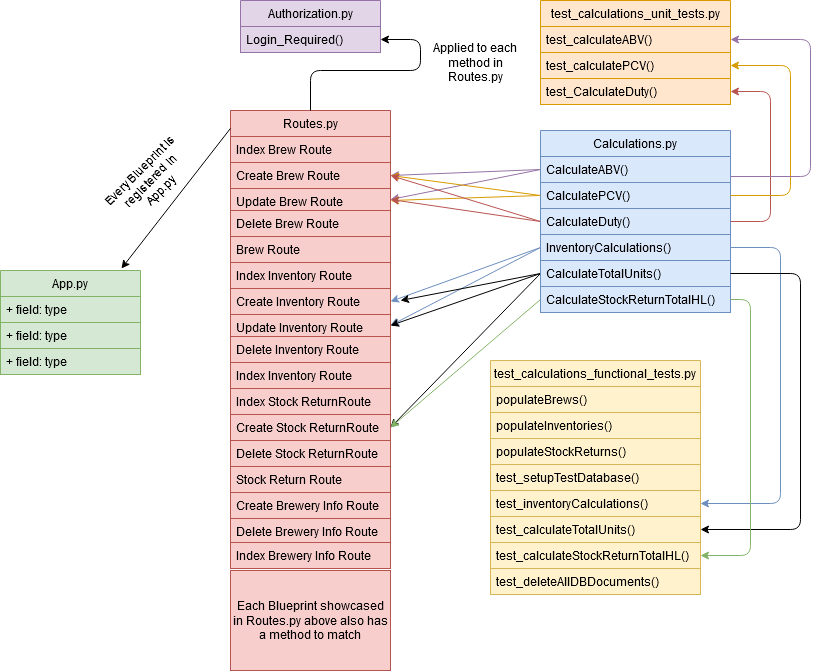
\includegraphics[width=1\textwidth]{Images/Server Class Diagram.png}
\end{figure}
\clearpage

\section{Cloud Servers}
The servers are the most integral part of the system as these allow communication between all parts of the project. The hosting service for the servers chosen was Heroku. This was due to providing a great free service which was important to the client. Other architectures may have been more suitable such as virtual machines on Amazon Web Services as response times would be more efficient and initial loading times would be greatly reduced, but in assessing the free tier options available Heroku seemed the correct choice. The API server is hosted on its own heroku server, this was done by creating a virtual environment for Flask with the necessary requirements and a procfile for information on running the Flask server e.g. gunicorn, a web server gateway which allows a larger volume of users than running using the the standard Flask server’s run method. The web application is also hosted on its own Heroku server. Both communicate with each other between the Heroku servers.\par
The project is to be deliverable to the client as a SaaS (Software as a Service). This means that the application is fully accessible to the client over their browser. This means no downloads or installations are required on the client side in order to use the application. As a result of this, technical issues, such as data, middleware, servers, and storage are all handled irrespective of the user. Delivering the software like this reduces cost on the company as they do not need to pay technicians to install software to computers. Also having the software accessible over the internet allows the user to access it from anywhere provided they have an internet connection. Another reason this was chosen was that it suits the company as the application may only be used once per month to record the revenue calculations. If the application was used on a daily basis then perhaps a local more stable (non-internet dependent) application may be more suitable.\par
SaaS is not perfect however, as it is internet dependent many issues such as performance levels and downtime periods may occur. This then leaves issues out of the users control as they have no backend access due to the application being controlled by a third party.

\section{Database}
The Database selected for the project was MongoDB. This seemed the best choice due to its rapid data insertion and retrieval. It also provides very specific and fast querying of data which is vital to the project due to the mass calculations needed for data on the server side which needed to access already stored database information. MongoDB uses BSON to store the database content on disk, which is a Binary form of JSON. The database however takes in information in JSON format and therefore no massive data conversion needs to take place which would further slow down the process. The database consists of three different collections for data in relation to figures, one for the brews, one for the inventories and another for stock returns. Another collection exists for storage of the user’s information which is used in warrant generation to fill out the necessary documentation. Each calculation collection can contain many documents which contain JSON data. However only one document exists in the brewery information collection as there should only exist one brewer's information at a time, when a change is made to the brewer information, the single document contained within in the collection is updated. Also a testing database using the same collections is set up in order to carry out the testing process without affecting real user data. The process of the data modeling can be seen in Figure \ref{fig:revenuecomp} of the Revenue Computation Process section.
\begin{figure}[h!]
 	\caption{Database Design Architecture}
	\label{image:databasedesign}
 	\centering
 	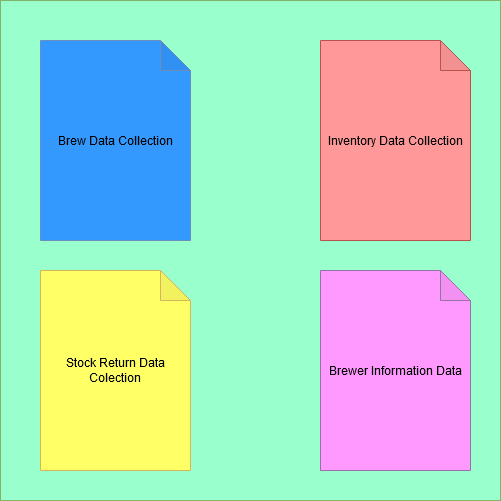
\includegraphics[width=0.9\textwidth]{Images/Database Structure.png}
\end{figure}